% chapter2_literature_review.tex

\section{Chapter Overview}
This chapter critically reviews literature relevant to \textbf{RootLens}, addressing RQ1 (what timing signals enable reliable classification) and RQ2 (what feature sets characterise sub-cause distinctions). The review covers five thematic areas: event-driven autoscaling delays in Kubernetes; existing RCA frameworks and their limitations, autoscaling challenges across cold start latency, scheduling delays, and metric propagation lag; a technological review of observability tools, dataset generation, and ML model selection; and a benchmarking framework informing the experimental design in Chapter~7. The chapter concludes by synthesising the research gap and articulating the contribution RootLens makes relative to surveyed literature.

\section{Concept Map}
Figure~\ref{fig:lit_concept_map} maps the four principal branches of the literature review: the Problem Domain (KEDA-triggered delays and three root cause categories), Existing Work (RCA frameworks, autoscaling challenges, cold start and scheduling studies), Technology (observability stack, ML techniques, dataset generation), and Evaluation (benchmarking metrics and comparative methodology).

\begin{figure}[H]
\centering
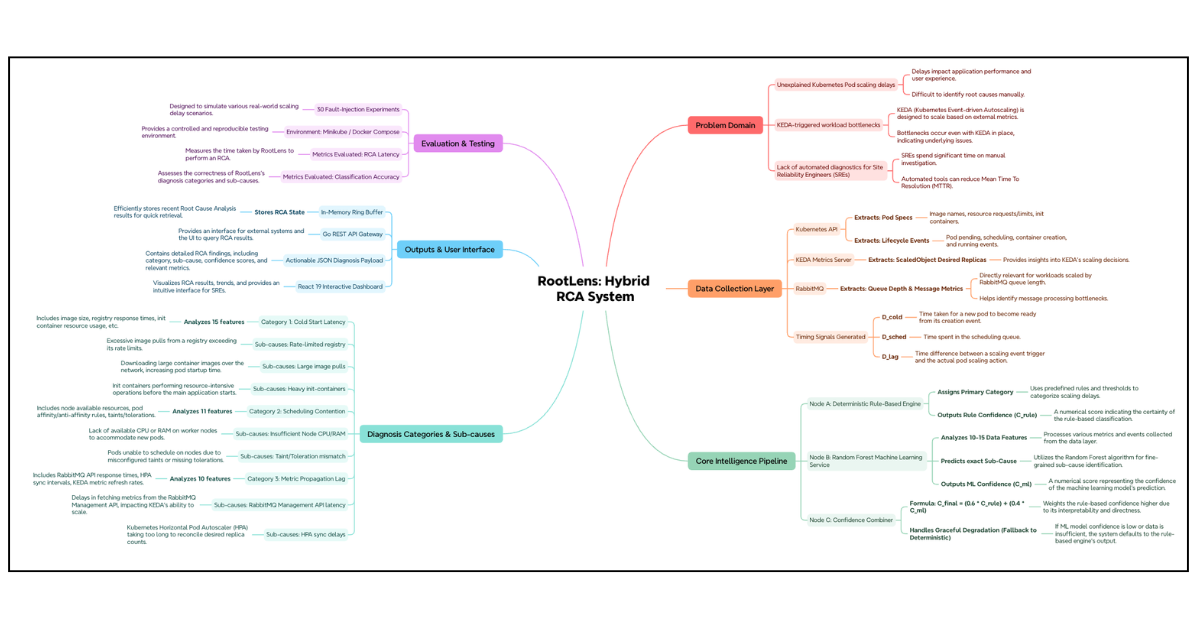
\includegraphics[width=1.0\textwidth]{thesis/assets/concept_map.png}
\caption{Concept Map of RootLens}
\label{fig:lit_concept_map}
\end{figure}

\section{Problem Domain}

\subsection{Overview of Event-Driven Autoscaling}
Kubernetes (Burns et al., 2016) provides the Horizontal Pod Autoscaler (HPA) for CPU/memory-based scaling, but HPA cannot respond to upstream event signals such as message queue depth. \textbf{KEDA} (KEDA Project, 2023) addresses this by watching configurable external scalers (RabbitMQ, Kafka, AWS SQS, etc.) and translating queue depth and message count metrics into HPA-compatible target replicas, enabling zero-to-$n$ scaling driven by business-relevant demand signals. The KEDA scaling loop introduces a timing chain spanning metric polling, HPA update, pod scheduling, image pull, and readiness probes, where failures at any step produce delays whose root cause may not be immediately obvious. Unlike HPA-based scaling where delays typically originate from pod startup, KEDA introduces additional latency sources upstream of pod creation in the metric polling and propagation stages, making diagnosis substantially more complex.

\subsection{Scaling Delay Categories}
Pelletier, Tundo and Tamburri (2020) conducted one of the few systematic analyses of autoscaling issues in cloud-native systems, corroborating the tripartite delay taxonomy adopted by RootLens without providing a diagnostic system or automated classification mechanism. Ilyushkin et al. (2017) quantified the relationship between pod startup latency and queue depth growth, establishing that cold start delays of even 30-60 seconds cause queue depth to exceed acceptable thresholds, directly motivating the operational urgency of rapid diagnosis. The SRE model (Beyer et al., 2016) identifies scaling failures as error budget risk requiring automated detection, while Nastic et al. (2020) emphasise that in event-driven contexts, latency violations compound non-linearly through downstream services, creating cascading failures that manual diagnosis cannot address within acceptable time bounds.

\begin{table}[H]
\centering
\begin{tabularx}{\textwidth}{|X|X|X|X|}
\hline
\textbf{Category} & \textbf{Cause} & \textbf{Key Signals} & \textbf{Research Gap} \\ \hline

Cold Start Latency & Image pull, container init, readiness delays & Pod start time, image pull duration & No real-time classification \\ \hline

Scheduling Delay & Resource constraints, affinity rules & Pod Pending duration, scheduling latency & Hard to distinguish sub-causes \\ \hline

Metric Propagation Lag & KEDA polling and Prometheus delay & Trigger vs event timestamps & Under-explored area \\ \hline

\end{tabularx}
\caption{Classification of Scaling Delay Categories}
\end{table}

\subsection{Observability and RCA Concepts}
Soldani and Brogi (2022) provide the most comprehensive survey of anomaly detection and RCA techniques for microservice applications, categorising approaches by detection method, diagnosis target, and evidence source. Their taxonomy identifies a gap in systems combining deterministic rules with ML-based sub-cause classification, precisely the hybrid approach adopted by RootLens. Notaro, Cardoso and Gerndt (2021) reinforce the distinction between symptoms (observable anomalies) and causes (underlying conditions), noting that most existing systems excel at symptom detection but struggle with causal attribution. Three fundamental challenges constrain automated RCA for autoscaling: \textbf{signal heterogeneity} across observability layers, \textbf{temporal alignment} across subsystems with different clock sources (Prometheus Authors, 2023), and \textbf{category overlap} where multiple delay types co-occur. None of the surveyed literature addresses all three simultaneously, constituting a significant gap that RootLens is designed to fill.

\section{Existing Work}

\subsection{RCA Frameworks}
Chen et al. (2019) proposed an ML-based outage prediction system using log features, metric anomalies, and change events, achieving high accuracy on general outage types but operating at coarser granularity than autoscaling delay diagnosis requires. A methodological limitation is their reliance on historical production data with retroactively assigned labels, introducing potential label noise when multiple failure modes co-occur; the RootLens fault-injection methodology avoids this through deliberate single-fault injection ensuring unambiguous ground-truth labels. Ma et al. (2020) developed AutoMap, a graph-based diagnosis framework using Prometheus metric correlation graphs for failure localisation. However, it requires a pre-built service dependency graph unavailable for failures occurring before application instantiation. Meng et al. (2020) proposed a causal inference approach using bidirectional causal models on metric time series, but it requires weeks of historical data for model construction and does not model pod lifecycle stages. Li et al. (2022) emphasised producing actionable diagnostics with sub-cause granularity mapping to remediation actions, aligning with the RootLens philosophy, but still assumes a running service topology.

All four frameworks share a structural limitation: they operate on application-layer telemetry (request traces, dependency graphs, metric time series) from running processes. Infrastructure-layer failures during image pull, pod scheduling, or container startup fall outside their diagnostic scope. RootLens targets precisely this class by operating on infrastructure-layer signals that exist before any application-layer telemetry is produced.

\begin{table}[H]
\centering
\begin{tabularx}{\textwidth}{|X|X|X|X|}
\hline
\textbf{Study} & \textbf{Approach} & \textbf{Strengths} & \textbf{Limitations} \\ \hline

Chen et al. (2019) & ML-based outage prediction & High accuracy & Coarse-grained, label noise \\ \hline

Ma et al. (2020) & Graph-based correlation & Effective localisation & Requires dependency graph \\ \hline

Meng et al. (2020) & Causal inference & Captures causal relationships & Needs historical data \\ \hline

Li et al. (2022) & Multi-source RCA & Actionable insights & Assumes running services \\ \hline

\end{tabularx}
\caption{Comparison of Existing RCA Frameworks}
\end{table}

\subsection{Autoscaling Challenges}
Toka, Varga and Marosi (2021) applied \textbf{Random Forest} classifiers to Kubernetes edge cluster scaling management, achieving over 90\% accuracy with sample sizes comparable to RootLens, demonstrating Random Forest's effectiveness for structured Kubernetes feature inputs. The comprehensive classifier comparison in Fern\'andez-Delgado et al. (2014), covering 179 classifiers across 121 datasets, independently confirms Random Forest's top-tier performance on structured tabular data. However, Toka et al.\ focus on proactive scaling decisions rather than reactive failure diagnosis. Pelletier, Tundo and Tamburri (2020) systematically catalogued autoscaling failure modes but provided only qualitative taxonomy without detection thresholds or automated classification. Qu, Calheiros and Buyya (2018) identified that interactions between scaling triggers and infrastructure constraints create qualitatively different failure modes, supporting the RootLens design of separate ML models per root cause category.

Taken together, these works address complementary but non-overlapping problems. Toka et al.\ (Toka, Varga and Marosi, 2021) ask what scaling action to take; Pelletier et al.\ (Pelletier, Tundo and Tamburri, 2020) ask what failures occur; Qu et al.\ (Qu, Calheiros and Buyya, 2018) ask how strategies interact with infrastructure. None asks why a specific scaling event failed, which is the diagnostic question operators face in production. RootLens bridges this gap by combining Pelletier's failure taxonomy with Toka's ML classification methodology.

\begin{table}[H]
\centering
\begin{tabularx}{\textwidth}{|X|X|X|X|}
\hline
\textbf{Study} & \textbf{Focus} & \textbf{Key Contribution} & \textbf{Gap} \\ \hline

Toka et al. (2021) & ML-based scaling & High prediction accuracy & No failure diagnosis \\ \hline

Pelletier et al. (2020) & Failure taxonomy & Categorisation of issues & No automation \\ \hline

Qu et al. (2018) & Scaling interactions & Infrastructure insights & No RCA capability \\ \hline

\end{tabularx}
\caption{Autoscaling Research and Identified Gaps}
\end{table}

\subsection{Cold Start Latency}
Wang et al. (2018) characterised cold start latency in serverless platforms, demonstrating that image pull duration, init container overhead, and readiness probe configuration are the primary determinants; their quantitative measurements informed the 15 features selected for the RootLens cold start explainer. Rattihalli et al. (2019) quantified pod cold start in Kubernetes specifically, validating the RootLens rule-based threshold ($D_{\text{cold}} > 30$s) and identifying discriminative sub-cause features. Notably, Wang et al.\ and Rattihalli et al.\ disagree on the relative importance of registry proximity versus image size, and RootLens includes both as features, allowing the Random Forest to learn relative importance empirically. Silva, Fireman and Pereira (2020) analysed container image optimisation techniques, and their characterisation of image-level factors informed the inclusion of estimated image size and registry response time as features.

A critical assessment reveals a field that has thoroughly characterised the phenomenon without progressing to diagnostic tooling. Wang et al., Rattihalli et al., and Silva et al.\ all operate within a measurement-and-optimisation paradigm where the goal is to quantify or reduce cold start latency, not to classify its cause at runtime. RootLens applies these characterisation findings directly into a 15-feature Random Forest classifier performing automated sub-cause classification in real time.

\subsection{Scheduling and Network Delays}
Burns et al. (2016) describe the Kubernetes scheduler as derived from the Borg system, where feasibility filtering failures were a documented operational challenge at scale. Carri\'on (2022) provide a comprehensive taxonomy of Kubernetes scheduling challenges, identifying resource fragmentation, affinity constraints, and topology-aware placement as recurring sources of scheduling delays; their taxonomy directly informed the sub-cause categories used in the RootLens scheduling explainer. RootLens uses the time between pod creation and node assignment ($D_{\text{sched}} = t_{\text{scheduled}} - t_{\text{created}}$) as the primary scheduling diagnostic signal. Basiri et al. (2016) introduced chaos engineering for proactively uncovering infrastructure weaknesses; their fault injection methodology was adopted for the RootLens dataset generation, enabling controlled reproduction of scheduling contention scenarios. Vayghan et al. (2021) identified that scheduling failures are among the hardest to diagnose manually because symptoms (pod stuck in Pending) are identical regardless of underlying cause (insufficient resources, affinity mismatch, or taint violation), directly motivating the need for ML-based sub-cause classification within this category.

\subsection{Metric Propagation Delays}
The KEDA polling architecture (KEDA Project, 2023) trades metric freshness against system load, while Prometheus (Prometheus Authors, 2023) uses a pull-based scrape model with a default 15-second interval. In combination, total metric propagation lag can reach 45-75 seconds in default configurations. RootLens quantifies this as $D_{\text{lag}} = t_{\text{keda\_trigger}} - t_{\text{queue\_event}}$. Unlike cold start and scheduling delays, metric propagation has received comparatively little research attention; most existing work on KEDA focuses on scaling policy correctness (Toka, Varga and Marosi, 2021) or performance evaluation (Ilyushkin et al., 2017) rather than diagnostic measurement. This makes the metric propagation category both the most novel RootLens contribution and the category with the smallest supporting literature. The RootLens ML explainer for this category uses 10 features, the fewest of the three models, reflecting the narrower feature space.

\section{Technological Review}

\subsection{Observability Stack}
The AIOps movement (Dang, Lin and Huang, 2019) identifies anomaly detection and RCA as the highest-value ML application areas for IT operations. Gulenko et al. (2018) demonstrate that distance-based clustering can detect anomalous behaviour from infrastructure metrics alone, supporting the RootLens design of operating on infrastructure-layer signals. Prometheus (Prometheus Authors, 2023) provides the observability foundation; RootLens leverages three specific integration points: the RabbitMQ exporter (queue depth at trigger time), the KEDA metrics endpoint (desired replica changes), and Kubernetes API server metrics (pod lifecycle timing). The Kubernetes Events API records pod lifecycle events with timestamps, and RootLens mitigates the one-hour default event retention and lack of guaranteed delivery ordering through timestamp-based correlation.

\subsection{ML Model Selection: Random Forest}
Toka, Varga and Marosi (2021) demonstrated Random Forest's high accuracy on structured Kubernetes management tasks, directly applicable to RootLens feature sets. Breiman (2001) established that Random Forest provides native feature importance scores through mean decrease in impurity, which RootLens uses for explainable diagnostics. Compared to alternatives (SVMs, gradient boosted trees, neural networks), Random Forest offers three advantages critical to the RootLens context: (1) strong performance with small training sets (34-42 samples per category), (2) robustness to feature scale differences, and (3) interpretable feature importance values supporting explainability. The trade-off is potentially weaker capture of complex non-linear interactions compared to gradient boosted methods, but for the low-dimensional feature spaces in RootLens this limitation is not expected to materially affect accuracy.

\subsection{Dataset Generation}
While Basiri et al. (2016) provide the methodological foundation for fault injection, a review of available literature reveals no existing labelled dataset for KEDA-triggered Kubernetes autoscaling delay classification. Datasets used by Chen et al. (2019) and Ma et al. (2020) contain application-layer metrics but lack the infrastructure-layer timing signals required by RootLens. Consequently, this research identifies the need to generate a novel ground-truth dataset through controlled chaos engineering to train and evaluate the proposed models, the methodology for which is detailed in Chapter 3.

\section{Benchmarking and Evaluation}

\subsection{Evaluation Metrics}
RootLens adopts four primary evaluation metrics: \textbf{root cause accuracy} ($\geq$95\% target) measuring correct category classification; \textbf{sub-cause accuracy} ($\geq$80\% target) measuring correct ML sub-cause classification; \textbf{mean RCA latency} ($<$300ms target) measuring wall-clock time from detection to classification; and \textbf{confidence calibration} measuring whether reported confidence scores reflect classification reliability. The calibration methodology draws on foundational work by Niculescu-Mizil and Caruana (2005), who demonstrated that well-calibrated classifiers produce probability estimates where stated confidence correlates monotonically with observed accuracy, and by Guo et al. (2017), who showed that model calibration is a distinct property from accuracy that must be assessed independently. Ilyushkin et al. (2017) established comparative evaluation methodology using controlled workload traces; RootLens adopts this by comparing the hybrid system against a \textbf{rule-only baseline} and an \textbf{ML-only baseline} across the same 30 fault-injection experiments, isolating each component's contribution.

\begin{table}[H]
\centering
\begin{tabularx}{\textwidth}{|X|l|X|}
\hline
\textbf{Metric} & \textbf{Target} & \textbf{Description} \\ \hline

Root Cause Accuracy & $\geq$95\% & Correct category classification \\ \hline

Sub-cause Accuracy & $\geq$80\% & ML classification accuracy \\ \hline

RCA Latency & $<$300ms & Diagnosis time \\ \hline

Confidence Calibration & High & Reliability of predictions \\ \hline

\end{tabularx}
\caption{Evaluation Metrics}
\end{table}

\section{Chapter Summary}
The literature converges on a structural gap: RCA systems (Ma et al., 2020; Meng et al., 2020; Chen et al., 2019; Li et al., 2022) assume running service topologies; autoscaling research (Toka, Varga and Marosi, 2021; Pelletier, Tundo and Tamburri, 2020; Qu, Calheiros and Buyya, 2018) splits between proactive optimisation and qualitative cataloguing; cold start studies (Wang et al., 2018; Rattihalli et al., 2019; Silva, Fireman and Pereira, 2020) characterise the phenomenon without diagnostic tooling. \textbf{No existing system provides automated, confidence-quantified root cause classification for KEDA-triggered Kubernetes scaling delays with sub-cause granularity.} RootLens fills this gap by combining Pelletier's failure taxonomy, Toka's ML methodology, and Rattihalli's cold start feature knowledge into a hybrid diagnostic engine. Chapter~3 describes the research methodology adopted to address this gap.